\documentclass[12pt, letterpaper]{article}
\usepackage[utf8]{inputenc}
\usepackage{geometry}
\usepackage{graphicx}
\usepackage{float}
\usepackage{amsmath}
\usepackage{amssymb}
\usepackage{fancyhdr}
\usepackage{lastpage}

% Page Geometry
\geometry{a4paper, total={170mm,257mm}, left=20mm, top=20mm}

% Header and Footer
\pagestyle{fancy}
\fancyhf{}
\rhead{Kaushik Vada \\ EE 134 - Digital IC Design \\ Homework 1 \\ \today}
\cfoot{Page \thepage \hspace{1pt} of \pageref{LastPage}}

\title{Homework 1}
\author{Kaushik Vada}
\date{\today}

\begin{document}

\maketitle

\section*{Problem 1.1}
\subsection*{Calculations}
The formula for the current is given by:
\[ I_D = \frac{1}{2} \mu C_{ox} \frac{W}{L} (V_{GS} - V_{th})^2 \]

\textbf{NMOS Current Calculation:}
\[ I_{D,n} = 0.5 \times 200 \times 10 \times (1.8 - 0.7)^2 \]
\[ I_{D,n} = 1000 \times (1.1)^2 \]
\[ I_{D,n} = 1000 \times 1.21 = 1210 \, \mu A \]
NMOS Current = \textbf{1210 $\mu A$}

\vspace{1em}

\textbf{PMOS Current Calculation:}
\[ I_{D,p} = 0.5 \times 80 \times 20 \times (1.8 - 0.9)^2 \]
\[ I_{D,p} = 800 \times (0.9)^2 \]
\[ I_{D,p} = 800 \times 0.81 = 648 \, \mu A \]
PMOS Current = \textbf{648 $\mu A$}

\subsection*{Analysis}
PMOS devices have wider channels because the mobility of holes ($\mu_p$) is lower than that of electrons ($\mu_n$). To match the current of an NMOS, the PMOS width must be increased.

\section*{Problem 1.2}
\begin{figure}[H]
    \centering
    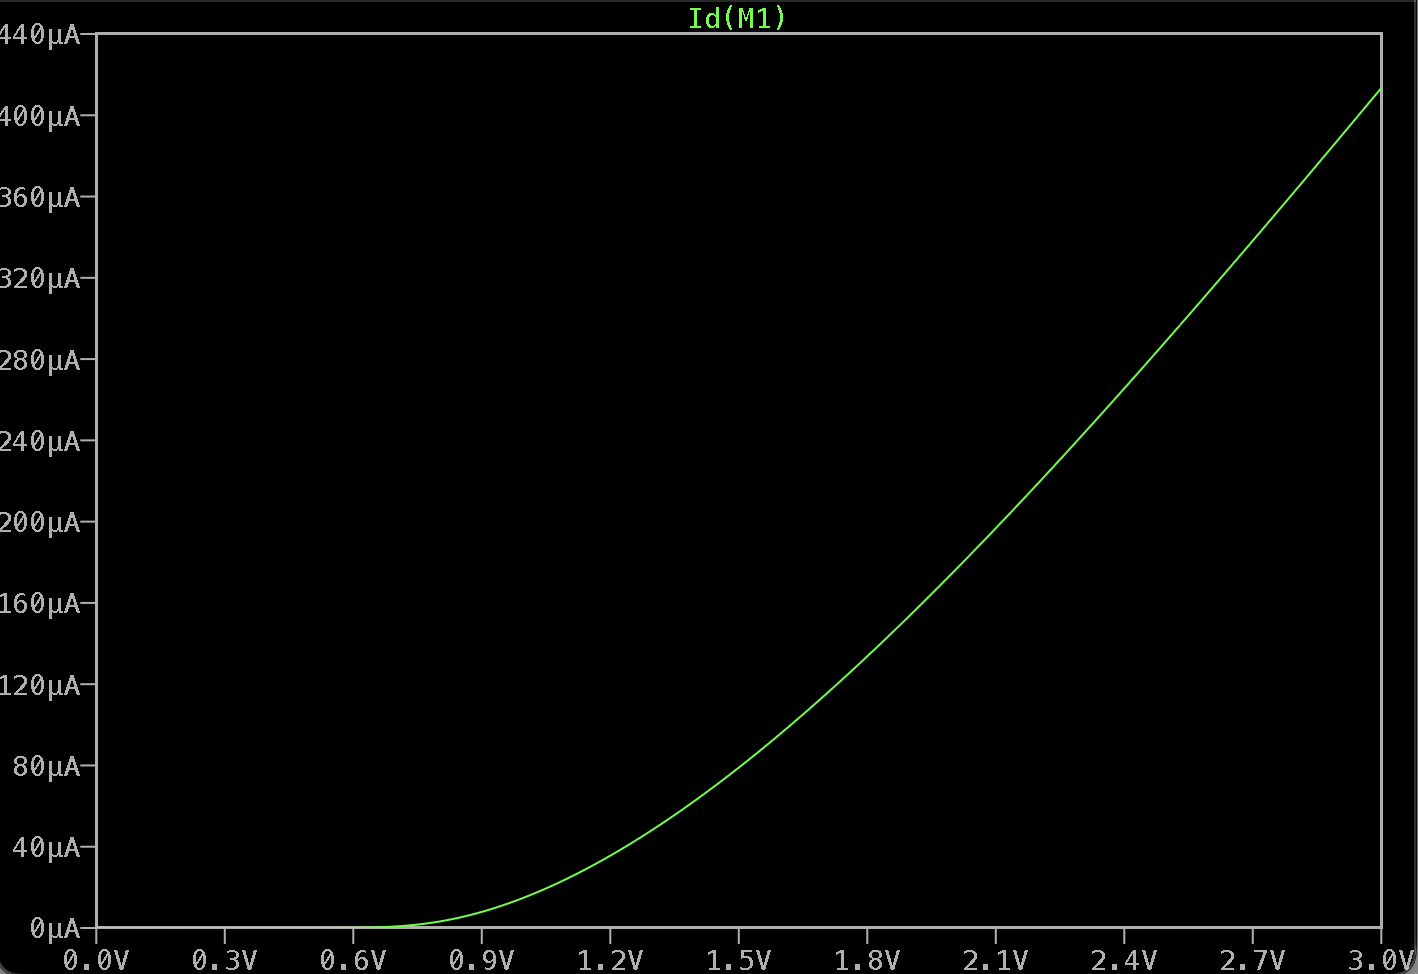
\includegraphics[width=0.8\textwidth]{Q1.2.png}
    \caption{Problem 1.2}
\end{figure}

\section*{Problem 1.3}
\begin{figure}[H]
    \centering
    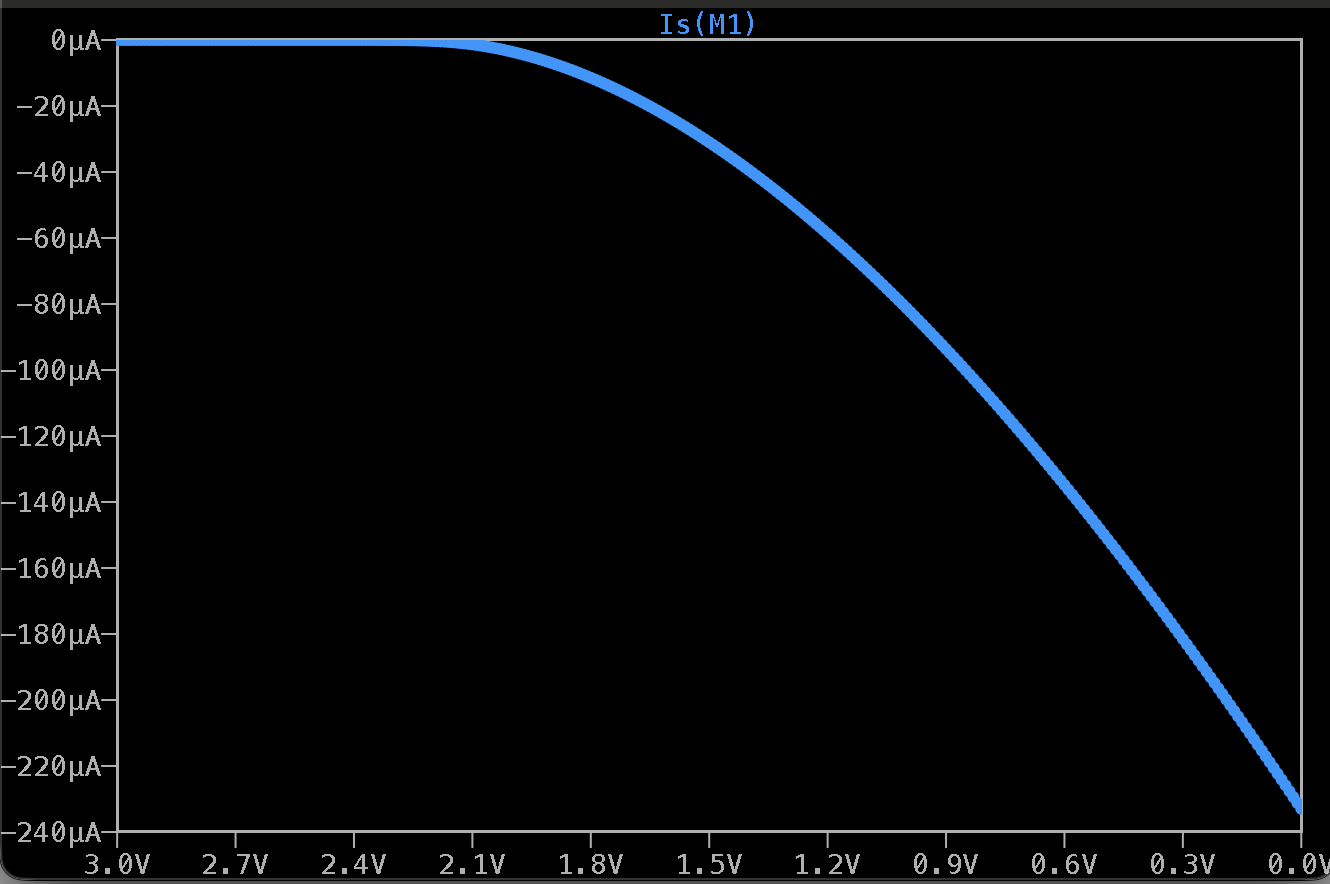
\includegraphics[width=0.8\textwidth]{Q1.3.png}
    \caption{Problem 1.3}
\end{figure}

\section*{Problem 1.4}
\begin{figure}[H]
    \centering
    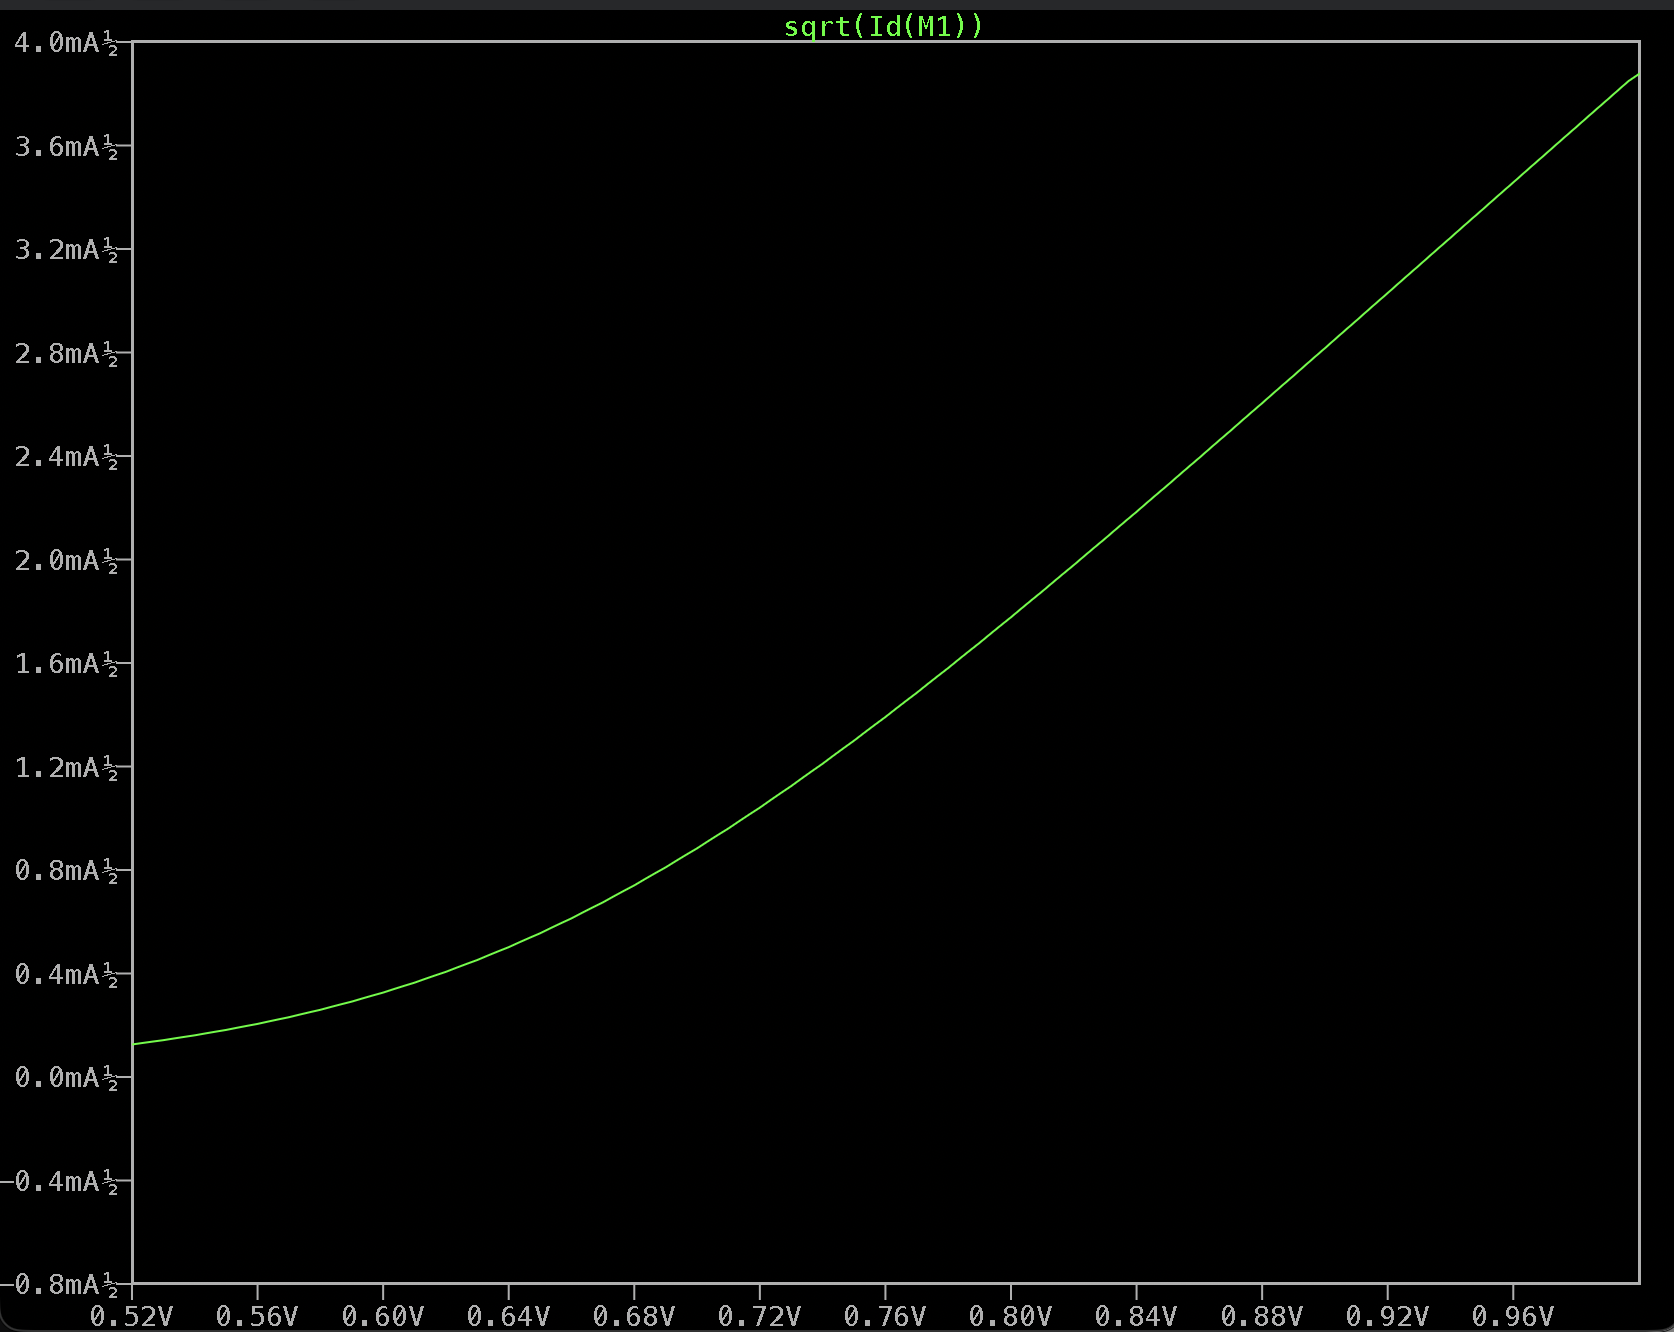
\includegraphics[width=0.8\textwidth]{Q1.4(a).png}
    \caption{Problem 1.4 (a)}
\end{figure}

\begin{figure}[H]
    \centering
    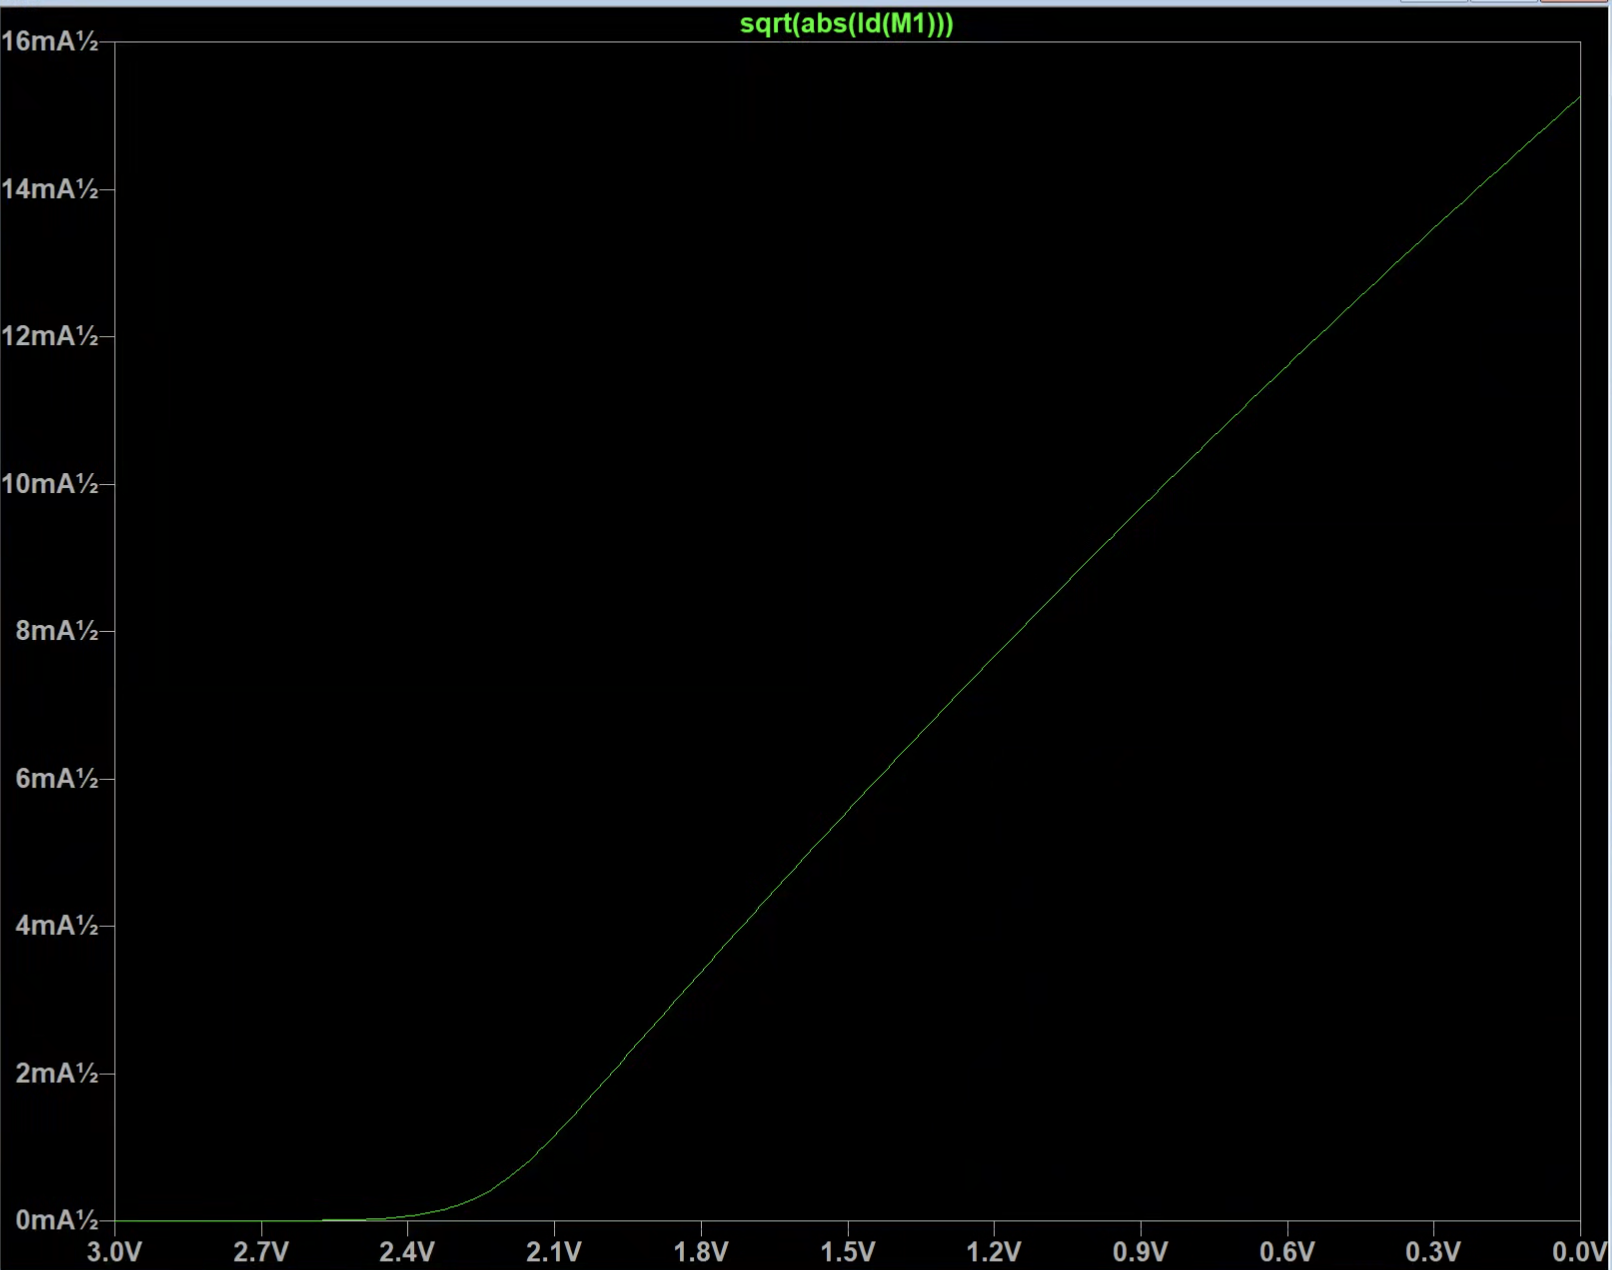
\includegraphics[width=0.8\textwidth]{Q1.4(b).png}
    \caption{Problem 1.4 (b)}
\end{figure}
Estimated NMOS $V_{th} = 0.726V$.

\section*{Problem 1.5}
\begin{figure}[H]
    \centering
    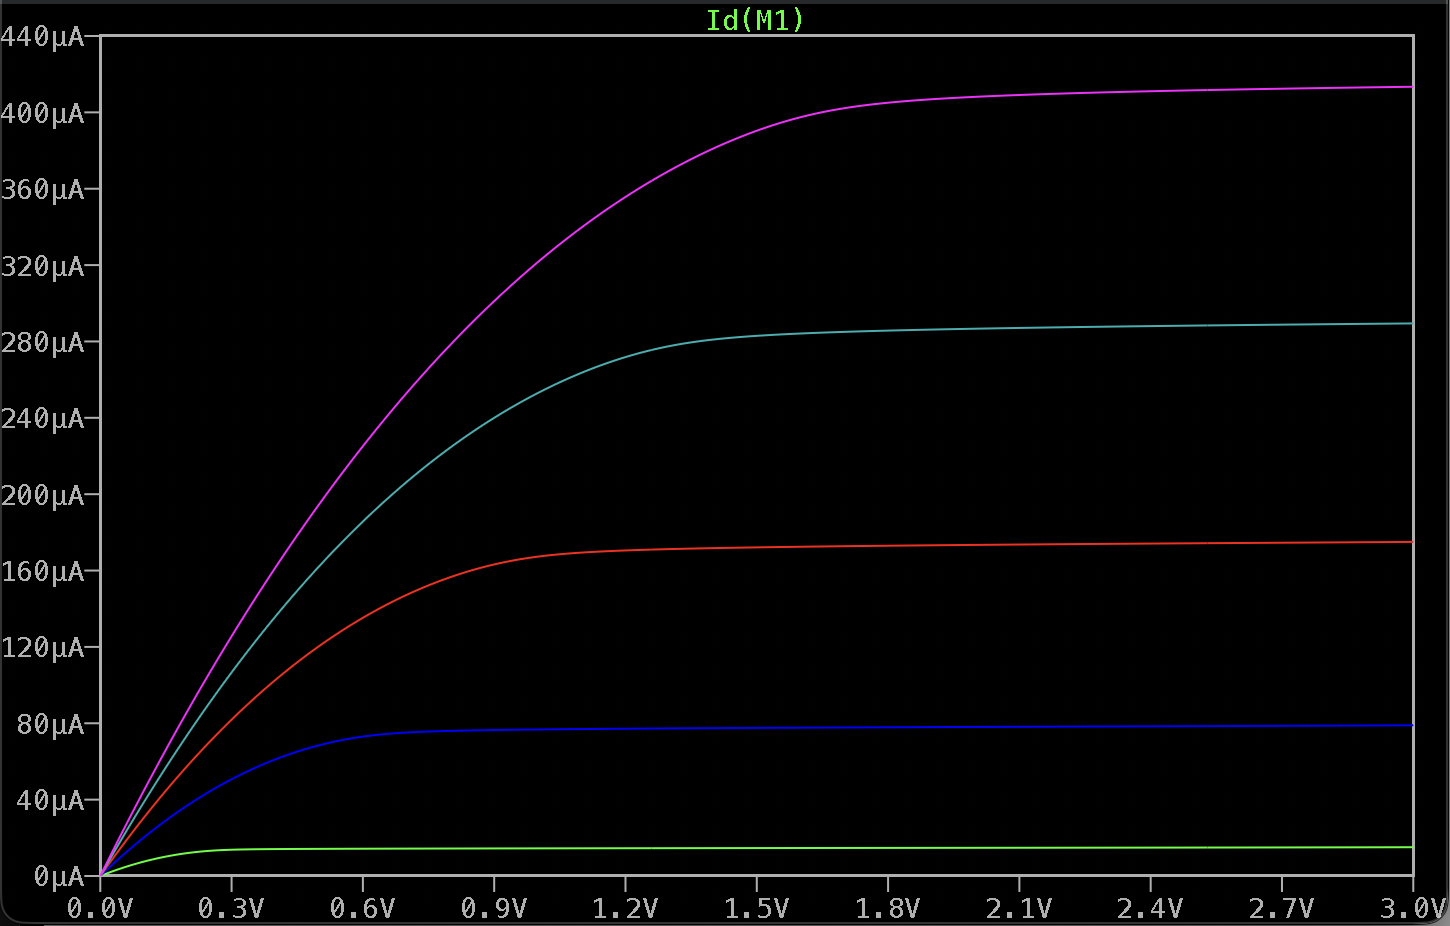
\includegraphics[width=0.8\textwidth]{Q1.5.png}
    \caption{Problem 1.5}
\end{figure}

\section*{Problem 1.6}
\begin{figure}[H]
    \centering
    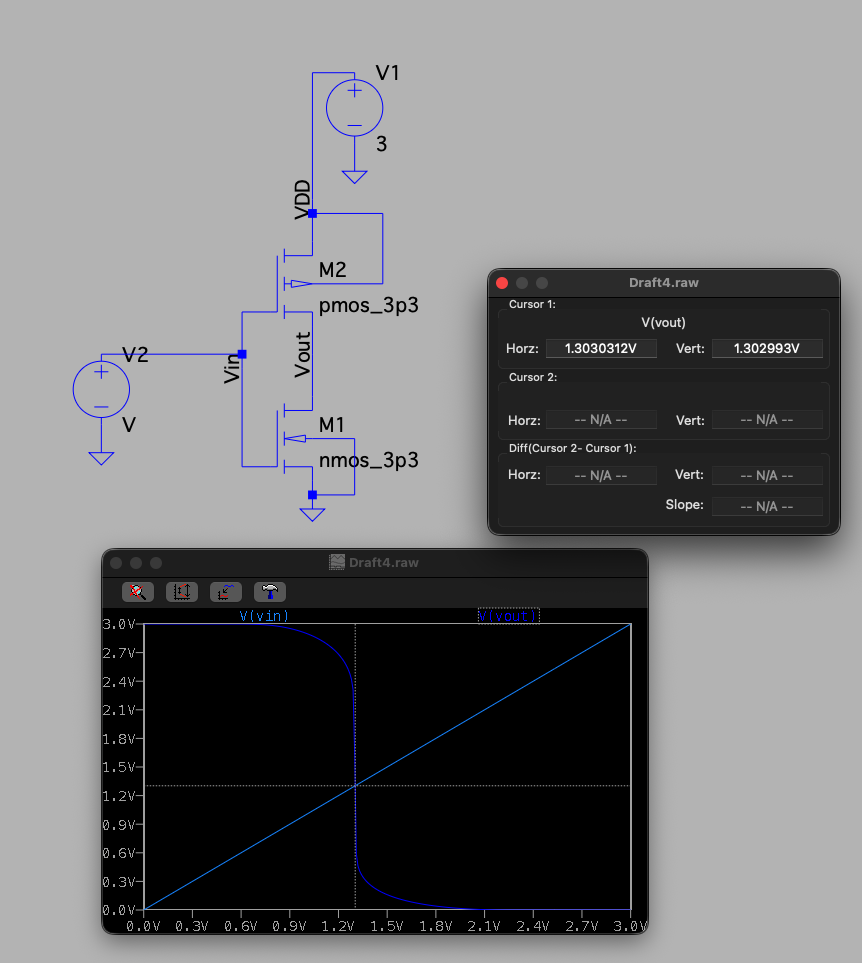
\includegraphics[width=0.8\textwidth]{Q1.6.png}
    \caption{Problem 1.6}
\end{figure}

\subsection*{Analysis: Why is the intersection not at 1.5V?}
The question asks why the intersection isn't exactly at half of $V_{DD}$ (1.5V).

\textbf{Explanation:} Even though the PMOS was made wider ($4\mu m$) than the NMOS ($2\mu m$), the NMOS is still "stronger."

\textbf{Reason:} Looking at the mobility values from Q1.1:
\begin{itemize}
    \item NMOS Mobility ($\mu_n$) $\approx 200$
    \item PMOS Mobility ($\mu_p$) $\approx 80$
\end{itemize}
The NMOS is roughly 2.5x faster than the PMOS, but the PMOS was only made 2x wider. Therefore, the NMOS is still slightly stronger, pulling the switching point lower than 1.5V.

\section*{Problem 1.7}
\begin{figure}[H]
    \centering
    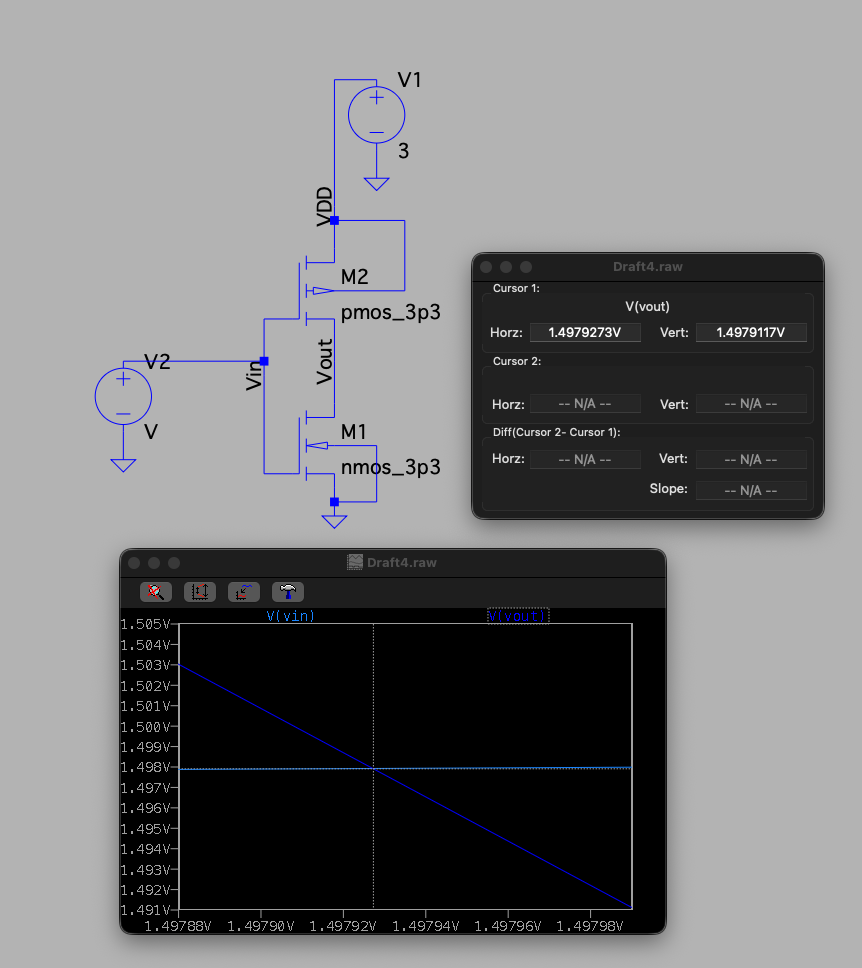
\includegraphics[width=0.8\textwidth]{Q1.7.png}
    \caption{Problem 1.7}
\end{figure}

\section*{Problem 1.8}
\begin{figure}[H]
    \centering
    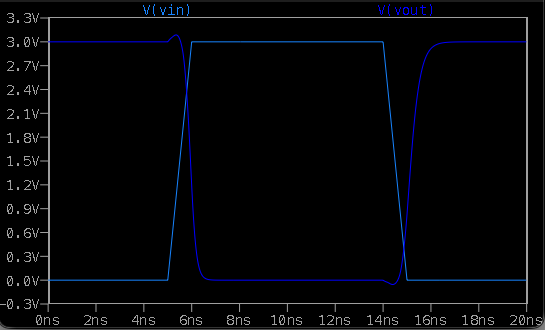
\includegraphics[width=0.8\textwidth]{Q1.8.png}
    \caption{Problem 1.8}
\end{figure}

\section*{Problem 1.9}
\begin{figure}[H]
    \centering
    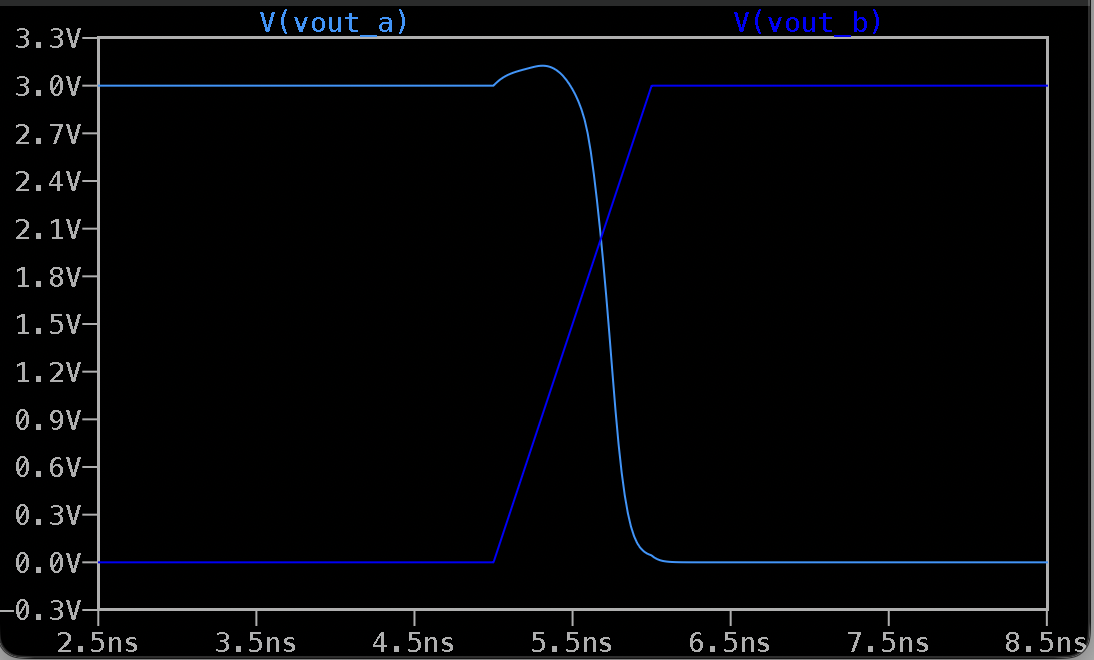
\includegraphics[width=0.8\textwidth]{Q1.9.png}
    \caption{Problem 1.9}
\end{figure}

\section*{Problem 1.10}
\begin{figure}[H]
    \centering
    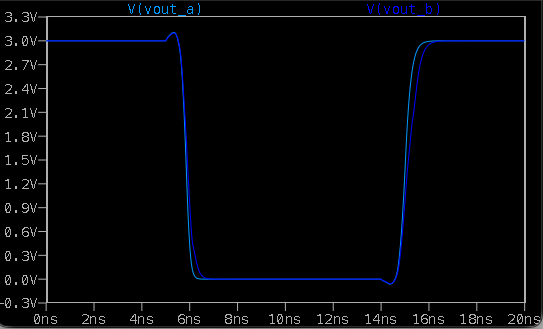
\includegraphics[width=0.8\textwidth]{Q1.10.png}
    \caption{Problem 1.10}
\end{figure}

\end{document}
